\documentclass{beamer}

\mode<presentation>
{
	\usetheme{CambridgeUS}
	\setbeamercovered{transparent}
}
\usepackage[spanish]{babel}
\usepackage[latin1]{inputenc}
\usepackage{color}
\usepackage{hyperref}
\usepackage{multicol}
\usepackage{algorithm,algorithmic}

\title[\textbf{ICI 4242 - Aut\'omatas y compiladores}]{\textbf{ICI 4242 - Aut\'omatas y compiladores}}

\subtitle{M\'aquina de Turing}

\author[Rodrigo Olivares]
{
	Rodrigo Olivares \\
	\vspace{0.5mm}
	Mg. en Ingenier\'ia Inform\'atica \\
	\vspace{0.5mm}
	\texttt{\normalsize rodrigo.olivares@uv.cl}
}

\institute[PUCV]

\date{1er Semestre} 

\subject{M\'aquina de Turing}

%\AtBeginSection
%{
%	\begin{frame}<beamer>
%	\frametitle{Contenido}
%	\tableofcontents[currentsection,currentsubsection]
%	\end{frame}
%}
%
%\AtBeginSubsection
%{
%	\begin{frame}<beamer>
%	\frametitle{Contenido}
%	\tableofcontents[currentsection,currentsubsection]
%	\end{frame}
%}

%\beamerdefaultoverlayspecification{<+->}

\begin{document}

	\begin{frame}
		\titlepage
	\end{frame}

	%\begin{frame}
	%	\frametitle{Contenido}
	%	\tableofcontents%[pausesections]
	%\end{frame}

	\section{M\'aquina de Turing}

		\subsection{Introducci\'on}

        \begin{frame}
            \frametitle{M\'aquina de Turing}
            \framesubtitle{Introducci\'on}

            \begin{exampleblock}{\textquestiondown Qu\'e es una M\'aquina de Turing?}
                Una M\'aquina de Turing es un \textbf{modelo matem\'atico}, propuesto por Alan Turing, que consiste en un aut\'omata capaz de implementar cualquier problema (funci\'on $f(x)$) matem\'atico expresado por medio de un \textbf{algoritmo}.
			\end{exampleblock}
		\end{frame}

%		\begin{frame}
%            \frametitle{M\'aquina de Turing}
%            \framesubtitle{Introducci\'on}
%
%            \begin{table}[H]
%                \begin{center}
%                    \begin{tabular}{|c|c|c|c|}\hline
%                        \textbf{Tipo} & \textbf{Lenguaje}       & \textbf{M\'aquina}   & \textbf{Gram\'atica} \\ \hline
%                                      & \textbf{Recursivamente} & \textbf{M\'aquina}   & \textbf{Sin}  \\
%                                    0 & \textbf{enumerable}     & \textbf{de Turing}   & \textbf{restricciones} \\ \hline
%                                      & Sensibles al            & Aut\'omata           & Dependiente del \\
%                                    1 & contexto                & linealmente acotados & contexto \\
%                                    & & & $\alpha$A$\beta$ $\rightarrow$ $\alpha \gamma \beta$\\ \hline
%                                      & Independiente del       & Aut\'omata           & Independiente del \\
%                                    2 & contexto                & de Pila              & contexto \\
%                                      &                         &                      & $A \rightarrow w$, $w \in (\Sigma,N)^{*}$\\ \hline
%                                      &                         & Aut\'omata           & Regular \\
%                                    3 &  Regular                & finito               & $A \rightarrow aB$\\ 
%                                      &                         &                      & $A \rightarrow a$\\\hline
%                    \end{tabular}
%                \end{center}
%            \end{table}
%		\end{frame}

        \begin{frame}
            \frametitle{M\'aquina de Turing}
            \framesubtitle{Introducci\'on}

            \begin{block}{Funcionamiento de una M\'aquina de Turing}
                \begin{itemize}
                    \item[$\rightarrow$] La M\'aquina de Turing tiene, un \textbf{control finito}, un \textbf{cabezal de lectura/escritura} y una \textbf{cinta} donde puede haber caracteres, y donde eventualmente viene la palabra de entrada.
                    \item[$\rightarrow$] La cinta es de longitud \textbf{infinita} hacia la izquierda y derecha, llen\'andose los espacios con el caracter blanco (que representaremos con \#).
                \end{itemize}
			\end{block}
		\end{frame}

        \begin{frame}
            \frametitle{M\'aquina de Turing}
            \framesubtitle{Introducci\'on}

            \begin{figure}[H]
                \begin{figure}
                    \begin{center}
                        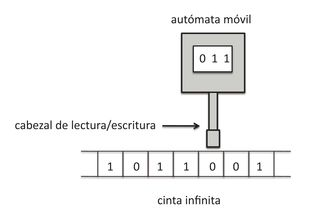
\includegraphics[scale=12]{images/mt.png}
                        \caption{M\'aquina de Turing}
                    \end{center}
                \end{figure}
            \end{figure}
		\end{frame}

        \begin{frame}
            \frametitle{M\'aquina de Turing}
            \framesubtitle{Introducci\'on}

			\begin{block}{Funcionamiento de una M\'aquina de Turing}
                \begin{itemize}
                    \item[$\rightarrow$] El cabezal de lectura/escritura de la M\'aquina de Turing, permite \textbf{leer} y \textbf{modificada} el s\'imbolo apuntado, durante la ejecuci\'on. 
                    \item[$\rightarrow$] El cabezal de lectura/escritura de la M\'aquina de Turing se mueve \textbf{bidireccionalmente} (\textbf{izquierda} y \textbf{derecha}), por lo que puede pasar repetidas veces sobre un mismo segmento de la cinta. En ocaciones, el cabezal procesa el s\'imbolo apuntado, per \textbf{no se mueve}.
                \end{itemize}
			\end{block}
		\end{frame}

%        \begin{frame}
%            \frametitle{M\'aquina de Turing}
%            \framesubtitle{Introducci\'on}
%
%			\begin{block}{Aut\'omata Finitos/Pila \emph{v/s} M\'aquina de Turing}
%                \begin{itemize}
%                    \item[$\rightarrow$] Los l\'imites de los aut\'omatas finitos y los aut\'omatas de pila vienen descritos por los lemas de bombeo.
%                    \item[$\rightarrow$] Lenguaje que no puede reconocer un aut\'omata finito: $$L=\{a^{n}b^{n}~|~n \in \mathbb{N}_{0}\}$$
%                    \item[$\rightarrow$] Lenguaje que no puede reconocer un aut\'omata de pila: $$L=\{a^{n}b^{n}c^{n}~|~n \in \mathbb{N}_{0}\}$$
%                \end{itemize}
%			\end{block}
%		\end{frame}

        \begin{frame}
            \frametitle{M\'aquina de Turing}
            \framesubtitle{Introducci\'on}

			\begin{block}{Definici\'on formal de una M\'aquina de Turing}
			    \begin{itemize}
                    \item[] Formalmente, una M\'aquina de Turing es una s\'eptupla $TM = \langle Q, \Sigma, \Gamma, \delta, q_{0}, \#, F)$, donde:
                    \begin{itemize}
                        \item[] $Q$: Conjunto de estados.
                        \item[] $\Sigma$: Conjunto de s\'imbolos terminales.
                        \item[] $\Gamma$: Conjunto de s\'imbolos de la cinta $(\Sigma \cup \gamma \cup \{\#\})$.
                        \item[] $\delta$: $Q \times \Gamma \rightarrow Q \times \Gamma \{\mathcal{L}, \mathcal{R}, \mathcal{S}\}$
                        \item[] $q_{0}$: Estado inicial
                        \item[] $\#$: Caracter de separaci\'on, vac\'io o blanco. Inicialmente, en las primera $n$ posiciones de la cinta est\'an $a_{1},a_{1},\ldots,a_{n}$. El resto de la cinta tiene s\'imbolos \#.
                        \item[] $F$: $F \subset Q$ conjunto de estados finales.
                    \end{itemize}
                \end{itemize}
			\end{block}
		\end{frame}

        \begin{frame}
            \frametitle{M\'aquina de Turing}
            \framesubtitle{Introducci\'on}

			\begin{block}{Al leer un s\'imbolo $a_{i}$, la MT puede:}
			    \begin{itemize}
                    \item[$\rightarrow$] Cambiar de estado.
                    \item[$\rightarrow$] Escribir un s\'imbolo $a_{j}$ en la cinta (en lugar de $a_{i}$).
                    \item[$\rightarrow$] Mover el cabezal hacia la izquierda ($\mathcal{L}$), a la derecha ($\mathcal{R}$) o en el mismo lugar ($\mathcal{S}$).
                \end{itemize}
			\end{block}
		\end{frame}

        \begin{frame}
            \frametitle{M\'aquina de Turing}
            \framesubtitle{Introducci\'on}

			\begin{block}{Descripci\'on instant\'anea:}
			    \begin{itemize}
                    \item[$\rightarrow$] Secuencia de la forma $\alpha_{1}q\alpha_{2}$ donde $\alpha_{1},\alpha_{2} \in \Gamma$ y $q \in Q$. Describe la situaci\'on de una M\'aquina de Turing.
                    \item[$\rightarrow$] La cinta contiene la cadena $\alpha_{1}\alpha_{2}$ seguida de infinitos blancos. El cabezal se\~nala el primer s\'imbolo de $\alpha_{2}$.
                \end{itemize}
			\end{block}
		\end{frame}

        \begin{frame}
            \frametitle{M\'aquina de Turing}
            \framesubtitle{Introducci\'on}

			\begin{block}{Descripci\'on instant\'anea:}
			    \begin{itemize}
                    \item[$\rightarrow$] Se dice que una M\'aquina de Turing (TM) acepta una cadena de entrada $w \in \Gamma$, si partiendo del estado inicial $q_{0}$ y en la cinta se encuentra la cadena $w$ seguida de blancos (\#), la m\'aquina TM procesa la cadena y termina en el estado de aceptaci\'on ($q_{f} \in F$).
                    \item[$\rightarrow$] Se define el lenguaje aceptado por una M\'aquina de Turing, $L(TM)$, como el conjunto de todas las cadenas $w$ aceptadas por la m\'aquina.
                    \item[$\rightarrow$] Los lenguajes aceptados por las M\'aquinas de Turing se denominan \textbf{recursivamente enumerables}.
                \end{itemize}
			\end{block}
		\end{frame}

        \subsection{Ejemplos}

        \begin{frame}
            \frametitle{M\'aquina de Turing}
            \framesubtitle{Ejemplos}

			\begin{exampleblock}{Ejemplos: (no incluye la cadena vac\'ia)}
			    \begin{itemize}
                    \item[$\rightarrow$] $L_{1}=\{a^{n}b^{n}~|~n \in \mathbb{N}\}$
                    \item[$\rightarrow$] $L_{2}=\{a^{n}b^{n}c^{n}~|~n \in \mathbb{N}\}$
                \end{itemize}
			\end{exampleblock}
		\end{frame}

        \begin{frame}
            \frametitle{M\'aquina de Turing}
            \framesubtitle{Ejemplo - Soluci\'on}

            \begin{figure}[H]
                \begin{figure}
                    \begin{center}
                        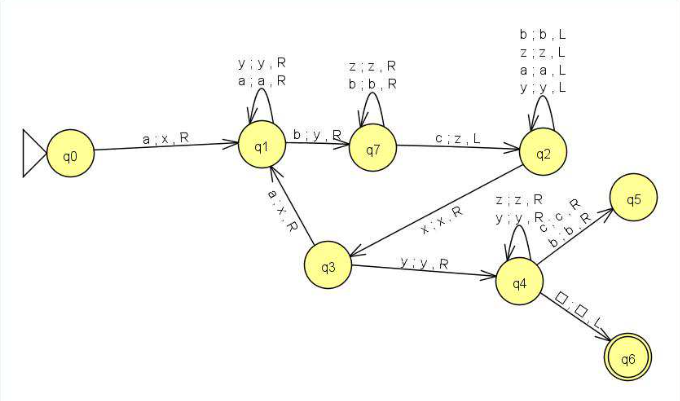
\includegraphics[scale=.5]{images/eje2.png}
                        %\caption{M\'aquina de Turing}
                    \end{center}
                \end{figure}
            \end{figure}
		\end{frame}

		\begin{frame}
			\frametitle{Preguntas}

			\hspace{4cm}\huge{Preguntas ?}
		
		\end{frame}
	\end{document}

\usetheme{default}
\usetheme{JuanLesPins}
\usetheme{Goettingen}
\usetheme{Szeged}
\usetheme{Warsaw}

\usecolortheme{crane}

\usefonttheme{serif}
\usefonttheme{structuresmallcapsserif}
 